\chapter{\IfLanguageName{dutch}{Stand van zaken}{State of the art}}
\label{ch:stand-van-zaken}

% Tip: Begin elk hoofdstuk met een inleidende paragraaf die beschrijft hoe
% dit hoofdstuk past binnen het geheel van de bachelorproef.
% Geef in het bijzonder aan wat de link is met het vorige en volgende hoofdstuk.

In dit hoofdstuk wordt de stand van zaken met betrekking tot ERP-systemen en patchmanagement behandeld. De focus ligt op het belang van patchmanagement binnen ERP-systemen, uitdagingen en strategieën die gepaard gaan met het beheren van patches in deze omgeving.

\section{Inleiding tot ERP-systemen en patchmanagement}
Enterprise Resource Planning (ERP) systemen zijn niet weg te denken van moderne bedrijfsvoering. Deze software speelt een essentiële rol bij het stroomlijnen en automatiseren van verschillende bedrijfsprocessen, variërend van financiën en voorraadbeheer tot human resources en klantrelatiebeheer.
Door het centraliseren van gegevens en processen helpen ERP-systemen organisaties om efficiënter te werken, betere beslissingen te nemen en hun concurrentiepositie te versterken. Met de toenemende afhankelijkheid van ERP-systemen komt ook de groeiende dreiging van cyberaanvallen. 

Als centrale systemen voor gevoelige bedrijfsgegevens, worden ERP-systemen vaak het doelwit van
kwaadwillende actoren die uit zijn op gegevensdiefstal, verstoring van bedrijfsprocessen of financieel gewin \autocite{Dekker2022}. In deze context wordt het belang van patchmanagement binnen ERP-systemen steeds groter, vooral om de veiligheid en stabiliteit van de systemen te waarborgen \autocite{Pearson2024}.
Het implementeren van een ERP-systeem is een evidente stap voor organisaties van een bepaalde omvang, meestal ergens rond een paar honderd werknemers. Zelfs sommige kleinere organisaties met complexe activiteiten zullen de noodzaak van ERP vinden. De vraag
naar ERP heeft een aanzienlijke markt gecreëerd. Volgens \textcite{Madh2024} was de wereldwijde ERP-softwaremarkt in 2023 \$49,80 miljard en wordt verwacht dat deze tegen 2030 zal stijgen naar \$140,14 miljard. Drie grote namen -
Microsoft, Oracle en SAP - domineren de markt, maar verschillende kleinere spelers bieden ook ERP-producten aan die op vele manieren concurrerend zijn met die van de marktleiders \autocite{Pratt2023}.

Patchmanagement verwijst naar het proces van het identificeren, beoordelen, testen en implementeren van softwarepatches om bekende kwetsbaarheden in systemen te verhelpen. Binnen het domein van ERP-systemen, is patchmanagement van groot belang
om de veiligheid en stabiliteit van de systemen te waarborgen. Door regelmatig patches toe te passen, kunnen organisaties potentiële beveiligingsrisico's minimaliseren en zichzelf beschermen tegen externe bedreigingen \autocite{Buenning2024}.

\section{Managed service providers}

Volgens \textcite{Gillis2021} is een en managed service provider (MSP) een extern bedrijf dat de IT-infrastructuur en eindgebruikerssystemen van een klant op afstand beheert. Bedrijven huren MSP's in om een pakket aan dagelijkse beheerdiensten uit te voeren (zoals patchmanagement). MSP's beheren
vaak dagelijkse diensten zodat klantorganisaties zich kunnen richten op het verbeteren van hun eigen diensten, zonder zich zorgen te hoeven maken over langdurige systeemuitval of onderbrekingen van de dienstverlening.
In de context van ERP-patchmanagement spelen MSP's een belangrijke rol voor hun klanten. ERP-systemen zijn complex en worden geïntegreerd met veel bedrijfsprocessen, het up-to-date houden van deze systemen is dus essentieel voor de beveiliging van bedrijven \autocite{Gillis2021}.

\section{Soorten patches}
Volgens \textcite{Buenning2024} zijn er drie types patches, namelijk beveiligingspatches, bugfixes en feature patches. Beveiligingspatches, die het aanpakken van nieuw ontdekte beveiligingskwetsbaarheden in het systeem inhouden, zijn een cruciaal
aspect van het handhaven van de integriteit en beveiliging van elke softwareomgeving. Naast beveiligingspatches spelen bugfixes ook een essentiële rol bij het zorgen
voor de soepele werking van softwaresystemen door problemen of fouten aan te pakken die zich kunnen voordoen in de functionaliteit van het systeem. Daarnaast zijn feature patches essentieel voor het verbeteren van de algehele prestaties van het systeem. Deze patches zijn bedoeld om de resource-eisen te
verminderen, de snelheid van toepassingen te verbeteren en nieuwe functionaliteiten te introduceren om de gebruikerservaring en efficiëntie te optimaliseren \autocite{Buenning2024}. \\

Binnen ERP-systemen moet de kern van het besturingssysteem, namelijk de kernel regelmatig gepatched worden, dit is dan met met één van de drie types patches. In ERP-systemen speelt de database ook een zeer belangrijke rol, hiervoor zij er ook regelmatig patches nodig. Deze patches zorgen er onder andere
voor dat de database optimaal blijft werken en dat data veilig blijft. Het is van belang voor organisaties om regelmatig de risico's te beoordelen en dus het implementeren van patches om de risico's te beperken en de soepele werking van hun systemen te garanderen.
Deze concepten worden weerspiegeld in het onderzoek van \textcite{Wrobel2023}, waarin het belang van patchmanagementstrategieën wordt benadrukt bij het aanpakken van beveiligingskwetsbaarheden, bugs en prestatieproblemen binnen softwareomgevingen.

\section{Patchmanagement vs Vulnerability management}
Volgens \textcite{Danby2023} is Patchmanagement specifiek gericht op het toepassen van patches om bekende kwetsbaarheden aan te pakken. Vulnerability management bevat een breder scala aan activiteiten. Deze activiteiten omvatten configuratiebeheer, beveiligingsbewustzijnstraining en penetratietesten, allemaal gericht op het verbeteren van de algehele beveiliging en het beheersen van risico’s.


\section{Trends en ontwikkelingen in  ERP en patchmanagement}

De eerste belangrijke trend is de nadruk op proactieve beveiligingsmaatregelen.
In een interview met \textcite{Munck2024} bleek dat in plaats van te wachten tot zich kwetsbaarheden voordoen, streven organisaties ernaar om potentiële beveiligingsrisico's voor te zijn door regelmatig patches toe te passen en beveiligingsupdates te implementeren.
Nog een belangrijke trend is dat ontwikkelingen binnen ERP bedrijven hebben geleid tot een groeiende afhankelijkheid van cloudservices voor patchmanagement.
Steeds meer organisaties verplaatsen hun ERP-systemen naar de cloud om te profiteren van schaalbaarheid, flexibiliteit en lagere operationele kosten.
Deze verschuiving naar de cloud heeft ook invloed op patchmanagement, aangezien organisaties nu op zoek zijn naar cloudgebaseerde oplossingen voor het beheren en implementeren van patches over hun gedistribueerde netwerken en apparaten \autocite{Kannan2023}. 

\section{Uitdagingen bij patching}
Organisaties worden geconfronteerd met verschillende uitdagingen bij het beheren van patches. Een van de meest voorkomende problemen is de traagheid waarmee updates worden uitgevoerd. Dit kan te wijten zijn aan verschillende
factoren, waaronder het gebrek aan middelen of prioriteitstoewijzing binnen de IT-afdeling. Als gevolg hiervan blijven systemen mogelijk kwetsbaar
voor bekende beveiligingsrisico's, wat de algehele veiligheid van het bedrijf in gevaar kan brengen \autocite{AppMaster2023}. 

Ook werken veel organisaties met meerdere systemen en toepassingen. Dit betekent dat IT-professionals verschillende besturingssystemen moeten kunnen patchen, zoals Linux (SUSE) waar de meeste ERP systemen op draaien, evenals verschillende applicaties van derden.
Het patchen van al deze systemen kan dus een hele klus zijn. Het patchen van systemen wordt vaak als tijdrovend en complex ervaren door IT- en beveiligingsprofessionals. Volgens \textcite{ivanti2021} vindt maar liefst 71\% van hen patchen te complex en tijdrovend. Het handmatig patchen van elk apparaat op een netwerk is niet alleen frustrerend en langzaam, maar
ook buitengewoon inefficiënt voor grotere organisaties. Dit leidt tot grote kosten voor bedrijven wanneer er moet gepatched worden, waardoor sommigen beroep doen op landen waar de kostprijs per werkuur veel lager ligt dan in België, zo kan men ook 's nachts patchen zonder nacht tarief te hoeven betalen \autocite{Munck2024}. 

Aangezien ERP-systemen vaak complexe architecturen hebben en geïntegreerd zijn met een breed scala aan andere systemen en applicaties, kunnen patches soms onverwachte problemen veroorzaken. Dit kan leiden tot verstoring van bedrijfsactiviteiten 
en downtime, wat op zijn beurt kan leiden tot financiële verliezen en reputatieschade voor het bedrijf.


\section{De keuze tussen handmatig en automatisch patchen}

Binnen organisaties die SAP ERP-systemen gebruiken, staan IT-teams vaak voor de keuze tussen handmatig of automatisch patchen. Beide benaderingen hebben hun eigen voor- en nadelen, het is cruciaal dat organisaties de juiste keuze maken op basis van hun specifieke behoeften en omgeving.

Handmatig patchen geeft IT-teams veel controle en flexibiliteit bij het beheren van patches in ERP systemen. Met deze aanpak kan elk patch-, klant- of server-combinatie afzonderlijk worden behandeld. Hierdoor kunnen alleen de 
noodzakelijke patches worden geïnstalleerd, precies wanneer dat nodig is, wat het risico op onbedoelde gevolgen vermindert. Compatibiliteitsproblemen kunnen worden verminderd en de algehele stabiliteit van het ERP-systeem wordt gewaarborgd \autocite{Hooper2018}.

Volgens \textcite{Hooper2018} is het grote nadeel van handmatig patchen dat de meeste patches moeten worden geïmplementeerd worden buiten de normale werkuren (weekends/'s nachts). IT-teams moeten voortdurend patchbulletins volgen, patches testen en implementeren, wat kan leiden tot vertragingen bij het 
toepassen van cruciale updates. Bovendien vergroot de menselijke factor het risico op fouten, waardoor organisaties kwetsbaar kunnen zijn voor beveiligingsrisico’s door gemiste patches of onjuiste implementaties. Automatisch patchen daarentegen biedt een hoog niveau van efficiëntie en consistentie bij het beheren van patches in ERP systemen. Met automatische patchingtools
kunnen patches toegepast worden volgens een vooraf ingesteld schema. Organisaties moeten ervoor zorgen dat ze de juiste patchingtools hebben geïmplementeerd die zijn afgestemd op hun specifieke behoeften en omgeving. Er bestaat ook het risico dat automatische patchingtools incompatibele patches toepassen, wat kan leiden tot systeemstoringen of conflicten met andere softwarecomponenten \autocite{Hooper2018}.

Volgens \textcite{Tozzi2017} is het beste om een evenwichtige updatestrategie te hanteren. Deze strategie maakt gebruik van automatische updates waar ze nuttig zijn, maar vermijdt ze in situaties waarin ze te veel risico met zich meebrengen
 of niet toereikend zijn. Updatestrategieën moeten natuurlijk worden afgestemd op de specifieke behoeften van de organisatie.

Over het algemeen zou een goed ontworpen updatestrategie automatische updates richten op kritieke beveiligingslekken, updates voor het besturingssysteem zelf en systemen die gemakkelijk kunnen teruggezet naar de oorspronkelijke staat. Aan de andere kant 
zijn updates voor firmware, randapparatuur, netwerkschakelaars en andere soorten software die niet betrouwbaar kunnen worden geautomatiseerd, evenals niet-kritieke updates en updates voor systemen die zeer beschikbaar moeten zijn, beter geschikt voor handmatige patching.
Deze aanpak helpt om een balans te vinden tussen up-to-date en veilig zijn aan de ene kant en de stabiliteit van uw software aan de andere kant.

\section{Wanneer patchen?}
Een kosten baten analyse wordt vaak gemaakt om te bepalen wanneer er gepatcht moet worden. Hier worden de kosten van het patchen afgewogen tegen de kosten van een eventuele cyberaanval.
In figuur ~\ref{fig:kostenbaten} van \textcite{Posey2024} zien we hoe de kosten baten analyse eruit kan zien.

\begin{figure}[h]
    \centering
    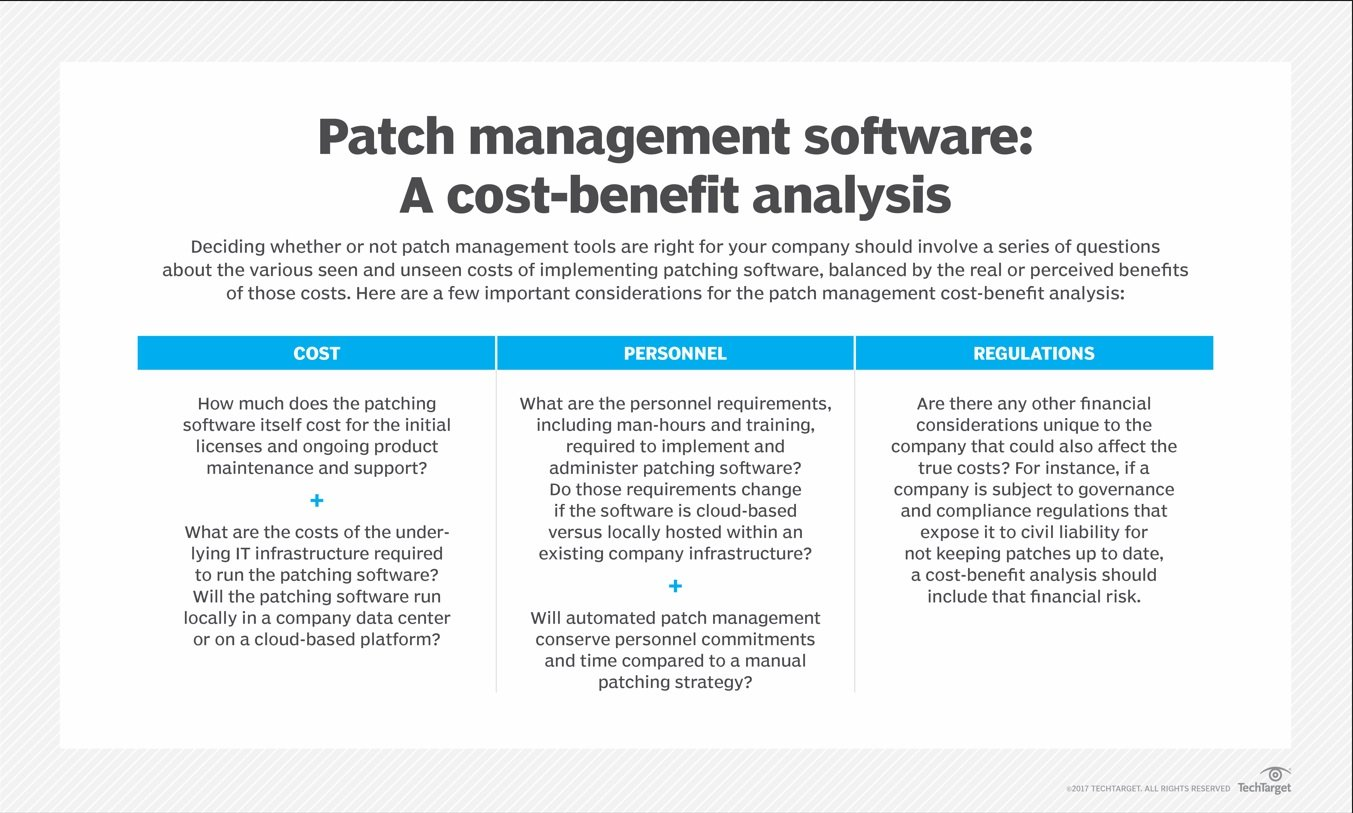
\includegraphics[width=\textwidth]{techtarget.jpg}
    \caption{Kosten baten analyse patching \autocite{Posey2024}}
    \label{fig:kostenbaten}
\end{figure}

\newpage

\section{Invloed van menselijke, technologische en organisatorische factoren op patchmanagement}




Patchmanagement binnen ERP-systemen wordt sterk beïnvloed door een combinatie van menselijke, technologische en organisatorische factoren. Het is belangrijk om dit te begrijpen voor een patchmanagementstrategie te ontwikkelen en te implementeren.


Technologische factoren omvatten de beschikbaarheid en kwaliteit van patchingtools en -technologieën binnen ERP-systemen. Geavanceerde
patchingtools kunnen het patchmanagementproces automatiseren en vereenvoudigen, waardoor de werklast voor IT-teams wordt verminderd en de kans op fouten wordt verkleind \autocite{Graffeo2018}.

Organisatorische factoren, zoals de samenwerking tussen verschillende afdelingen en de implementatie van duidelijke patchmanagementprocedures, zijn ook van groot belang. Een goed gestructureerd patchmanagementbeleid, ondersteund door heldere communicatiekanalen en 
duidelijke verantwoordelijkheden, kan de efficiëntie van het patchmanagementproces aanzienlijk verbeteren. Door nauw samen te werken met verschillende belanghebbenden, waaronder IT-teams, beveiligingsexperts en operationele afdelingen, kunnen organisaties ervoor 
zorgen dat patching prioriteit krijgt en effectief wordt uitgevoerd​ \autocite{Maditinos_2011}.

Ook menselijke factoren spelen een cruciale rol in het patchmanagementproces. Het bewustzijn van medewerkers over de noodzaak van patching en het belang van cybersecurity
is van vitaal belang. Zonder voldoende bewustwording kunnen patches over het hoofd worden gezien of niet tijdig worden toegepast, waardoor de veiligheid van het ERP-systeem in gevaar komt.

Het succesvol beheren van patches vereist daarom een holistische benadering waarbij rekening wordt gehouden met zowel menselijke, technologische als organisatorische factoren.
Door bewustwording te vergroten, medewerkers te trainen, geavanceerde tools te gebruiken en effectieve samenwerking te bevorderen, 
kunnen organisaties hun SAP ERP-systemen adequaat beschermen tegen potentiële bedreigingen en de operationele continuïteit waarborgen.

\section{Strategieën voor minimalisering van de impact op de continuïteit}
Bij het implementeren van patches binnen SAP ERP-systemen is een zorgvuldige planning cruciaal. Voer patchactiviteiten uit tijdens niet-kritieke periodes, zoals buiten kantooruren, om verstoring te minimaliseren. Een gefaseerde implementatie waarbij eerst minder kritieke systemen worden gepatcht, helpt
 compatibiliteitsproblemen vroegtijdig te identificeren. Fallbackstrategieën moeten voorzien worden, zoals het maken van back-ups, om snel te kunnen reageren op onvoorziene problemen en zo indien nodig terugkeren naar de staat voordien. Deze aanpak minimaliseert de impact op de operationele continuïteit en waarborgt de veiligheid en stabiliteit van SAP ERP-systemen \autocite{Shein2022}.

\section{Communicatiestrategieën voor belanghebbenden}
Heldere en tijdige communicatie met belanghebbenden over geplande patchactiviteiten is van vitaal belang. Volgens \textcite{Toren2019} essentieel om begrijpelijke informatie te verstrekken over de redenen achter het patchen,
mogelijke impact en benodigde voorzorgsmaatregelen. Daarnaast zijn het opzetten van communicatiekanalen voor feedback en het bieden van ondersteuning aan gebruikers eveneens cruciaal voor een succesvolle implementatie.


\section{Cloudgebaseerde ERP-systemen}
Volgens \textcite{Forbes2021} kan de cloud een meer gestroomlijnde benadering bieden, terwijl tegelijkertijd geprofiteerd wordt van beveiligings best practices en updates van cloud- en softwareleveranciers. Ook bieden volgens \textcite{Ruiter2024}
cloudgebaseerde ERP-systemen verschillende voordelen ten opzichte van traditionele on-premises oplossingen. Ze kunnen gemakkelijk de infrastructuur schalen met de groeiende behoeften van een organisatie, 
vereenvoudigen het implementatieproces van beveiligingspatches en bieden realtime zichtbaarheid in de patchstatus van alle apparaten, ongeacht hun locatie. De initiële kosten zijn lager bij de cloudinfrastructuur, en
deze kosten zijn ook meer voorspelbaar, terwijl bij een on-premise ERP-systeem de initiële kosten veel hoger kunnen zijn, maar de
totale kosten na verloop van tijd lager kunnen uitvallen, afhankelijk van de vereisten. Een ander voordeel van de cloudprovider is dat
de verantwoordelijkheid voor data beveiliging nu ook bij hen ligt. De interesse in ERP
overstijgt verticale industrieën, met fabrikanten, dienstverleners, non-profitorganisaties en overheidsentiteiten die allemaal behoefte hebben aan de mogelijkheden ervan om efficiënt en effectief te kunnen
functioneren. Bedrijven over de hele wereld vertrouwen nu steeds meer op cloud computing om hun bedrijf te runnen. Het groeit zo snel in populariteit dat minder dan een derde van de bedrijfsapplicaties nog verwacht wordt 
te worden gehost op traditionele servers tegen 2022, en de rest zal vertrouwen op cloud computing-oplossingen \autocite{Pimentel2017}.
Patchmanagement in cloudgebaseerde ERP-systemen is dus een steeds belangrijker wordend aspect van IT-beheer voor moderne organisaties. Met de opkomst van cloud computing hebben veel bedrijven ervoor gekozen
om hun ERP-systemen naar de cloud te verplaatsen om te profiteren van de schaalbaarheid, flexibiliteit en kosteneffectiviteit die de cloud biedt. 
Met de juiste aanpak kunnen organisaties de beveiliging en betrouwbaarheid van hun cloudgebaseerde ERP-systemen waarborgen in een snel evoluerend technologisch landschap.

\section{De toekomst van patchmanagement}
De toekomst van AI in patchmanagement ziet er veelbelovend uit, vooral met de groeiende uitdagingen waar organisaties mee te maken hebben bij
het beheren van patches. Elke week worden er steeds meer patches uitgebracht, wat het moeilijk maakt om te bepalen welke patches moeten worden toegepast, hoe snel dat moet gebeuren en waar. Dit zorgt voor een aanzienlijke werklast voor patchmanagementprogramma's, die nog verder toeneemt naarmate
organisaties meer eindpunten en diverse softwarebronnen toevoegen. Volgens \textcite{OFlaherty2023} wenden steeds meer bedrijven zich tot AI en machine learning
om deze uitdagingen aan te pakken. Deze technologieën kunnen helpen bij het detecteren, prioriteren en snel toepassen van patches wanneer dat nodig is. Dit leidt tot een efficiëntere werking, waardoor de algehele beveiliging wordt verbeterd door kwetsbaarheden sneller te 
identificeren en de kans te verkleinen dat deze worden uitgebuit in aanvallen.
Ook zegt OFlaherty dat AI-algoritmen begrijpen de complexe relaties tussen verschillende variabelen en kunnen een patchschema aanbevelen dat is afgestemd op de specifieke behoeften van een organisatie. Daarnaast kunnen AI-tools compatibiliteitsrisico's 
verminderen door slimme implementatietests uit te voeren en de belasting van IT-resources te verlagen. Met AI kunnen bedrijven ook
 endpoint- en gebruikersprofielen evalueren, zodat alleen relevante patches op het juiste moment worden toegepast, met minimale impact op gebruikers en bedrijfsactiviteiten. Hoewel de toepassing van AI in patchmanagement veel potentieel heeft, zijn er 
 ook uitdagingen en risico's. Het gebruik van AI in patchmanagement is nog nieuw en organisaties moeten een steile leercurve doorlopen om deze technologie effectief te implementeren. Bovendien zijn er ethische 
overwegingen bij het gebruik van AI voor autonome beslissingen over patchprioritering en -implementatie. AI is niet perfect en de voorspellingen zijn niet altijd nauwkeurig, wat kan leiden tot fouten bij het beoordelen van de impact van patches​ \autocite{OFlaherty2023}.

\section{Patchmanagement best practices}
Om patchmanagement effectief te kunnen implementeren binnen een organisatie zijn bepaalde stappen noodzakelijk. Volgens \textcite{Robb2023} zou een uitgebreide beoordeling van alle 
ERP-systemen of -programma's zou voor een bedrijf zeer nuttig blijken. Dit maakt de identificatie van ontbrekende patches mogelijk op basis van hun 
ernstniveaus en zorgt ervoor dat prioriteiten kunnen worden gesteld. Vervolgens zegt \textcite{ManageEngine2024} dat de planning van patch-implementaties cruciaal: deze moeten worden 
georganiseerd zonder nadelige gevolgen voor de productiviteit van werknemers, doorgaans door afzonderlijke implementatieschema's te gebruiken voor verschillende 
afdelingen of systemen die elkaar niet hinderen. Een patchbeheerprogramma bestaat doorgaans uit tools die automatisch patches kunnen implementeren op basis 
van de beschikbaarheid van de gebruiker en de uptime van het systeem. Naast de strategieën die zijn ontwikkeld om alle programma's te patchen, zijn het 
testen van patches na de implementatie en het garanderen van een roll-back-mogelijkheid voor patches voor het geval ze problemen veroorzaken ook noodzakelijke 
stappen voor een effectief patchbeheerproces. Het is van cruciaal belang om een ​​centraal punt voor de patchbeheeroplossing te selecteren, de nadruk te leggen 
op de patches die moeten worden geïmplementeerd en op het patchproces. \autocite{ManageEngine2024}


